\newpage
\section{Aktivierungsfunktionen}
Die Aktivierungsfunktion entscheided ob ein Neuron aktiviert wird oder nicht \cite{nwankpa2018activation}.
Sie können entweder linear oder nicht-linear sein.
Es ist aber nötig nicht-lineare Funktionen zu verwenden, damit jede kontinuierliche Funktion approximiert werden kann \cite{apicella2021survey}.
Sie unterscheiden sich in ihren Eigenschaften und Berechnungskosten, was eine besondere Rolle für Mikrocontroller spielt.
\newline
\newline
In der frühen Geschichte der neuronalen Netzwerke wurde die \textit{Sigmoid}-Funktion (\ref{formular:af_sigmoid}) viel verwendet, da sie asymptotisch begrenzt,
kontinuierlich und nicht-linear ist \cite{apicella2021survey}.
Heute wird sie oft in der Ausgabeschicht für binäre Klassifizierungsprobleme eingesetzt \cite{nwankpa2018activation}.
Allerdings ist sie für tiefe neuronale Netzwerke ungeeignet, da der Gradient zwischen 0 und 0.25 ist und dadurch im
Backpropagation-Prozess bereits nach wenigen Schichten gegen 0 geht.
Die \textit{SoftMax}-Funktion (\ref{formular:af_softmax}) oder normalisierte Exponentialfunktion berechnet für einen Eingabevektor eine Wahrscheinlichkeitsverteilung.
Die Einträge dieser Verteilung können für die Wahrscheinlichkeiten der einzelnen Klassen eines multivariat Klassifizierungsproblem interpretiert werden.
\begin{align}
    \label{formular:af_sigmoid}
    \text{sigmoid}(x) = \frac{1}{1 + e^{-x}}
\end{align}
\begin{align}
    \label{formular:af_softmax}
    \text{softmax}(x_i) = \frac{e^{x_i}}{\sum_j e^{x_j}}
\end{align}
\subfigbox{
\subfigure[Sigmoid/SoftMax]{\label{subfig:af_sigmoid}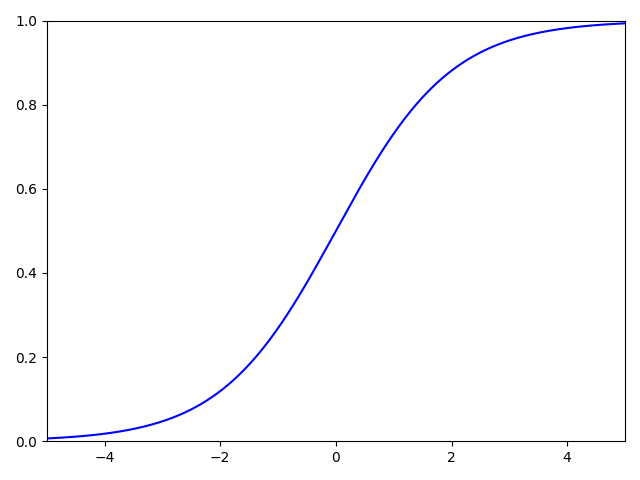
\includegraphics[width=0.495\linewidth]{images/activation_function_heaviside.png}}\hfill%
\subfigure[ReLU Varianten]{\label{subfig:af_relu}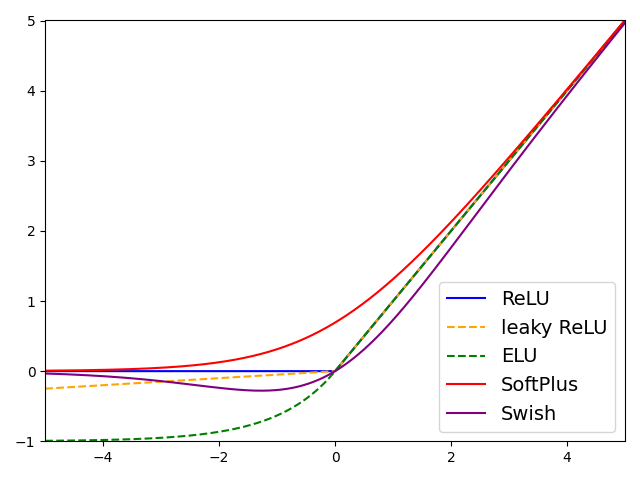
\includegraphics[width=0.495\linewidth]{images/activation_function_relu_varianten.png}}
}{Für diese Arbeit relevante Aktivierungsfunktionen.}{fig:activation_functions}
\newline
\newline
Zur \textit{ReLU}-Familie \cite{apicella2021survey} gehört die ReLU-Funktion \cite{glorot2011deep, konda2014zero, elfwing2018sigmoid, alcaide2018swish} und
ihre Varianten \cite{maas2013rectifier}, sowie die \textit{SoftPlus}- \cite{dugas2001incorporating} und \textit{Swish}-Funktion \cite{ramachandran2017searching}.
ReLU (\ref{formular:af_relu}) steht für \glqq\textit{rectified linear function}\grqq\ und wird häufig in modernen neuronalen Netzwerken verwendet \cite{apicella2021survey}.
Sie ist nicht differenzierbar bei 0 und die Ableitung für negative Eingaben ist 0.
Dies kann zu \textit{sterbenden Neuronen (engl. dying neurons)} führen, da der Bias so negativ wird, sodass das Neuron nicht mehr aktiviert wird.
Zudem ist der Trainingsprozess verlangsamt, wenn der Gradient konstant 0 ist.
Dafür ist die Ableitung der Funktion ansonsten 1, was den Backpropagation-Prozess vereinfacht, da der Gradient neutral zur Aktivierungsfunktion ist.
\begin{align}
    \label{formular:af_relu}
    \text{ReLU}(x) = \max(x, 0)
\end{align}
Varianten sind beispielsweise \textit{leaky ReLU} \cite{maas2013rectifier} (\ref{formular:af_leaky_relu}) und \textit{ELU (exponential linear unit)} (\ref{formular:af_elu})
\cite{clevert2015fast}, welche versuchen die Defizite des konstanten 0 Gradienten zu lösen, indem der negative Teil der Funktion nicht 0 ist.
\begin{align}
    \label{formular:af_leaky_relu}
    \text{leaky\_ReLU}_{\alpha}(x) = \begin{cases}
                               x & \text{, wenn } x \geq 0\\
                               \alpha x & \text{, ansonsten } (\alpha\in \mathbb{R}_{0}^{+})
    \end{cases}
\end{align}
\begin{align}
    \label{formular:af_elu}
    \text{ELU}_{\alpha}(x) = \begin{cases}
                                 x & \text{, wenn } x \geq 0\\
                                 \alpha(e^{x} - 1) & \text{, ansonsten } (\alpha\in \mathbb{R}_{0}^{+})
    \end{cases}
\end{align}
\textit{SoftPlus} (\ref{formular:af_softplus}) ist analytisch, dafür im Vergleich zu ReLU aufwendiger zu berechnen ist\cite{apicella2021survey}.
\begin{align}
    \label{formular:af_softplus}
    \text{softplus}(x_i) = \ln(e^x + 1)
\end{align}
Eine weitere Variante ist \textit{Swish} \cite{ramachandran2017searching} (\ref{formular:af_swish}).
Sie ist analytisch aber nicht monoton.
Im Vergleich zu ReLU ist sie aufwendig zu berechnen.
Ihre Autoren behaupten aber, dass dadurch bessere Ergebnisse erzielt werden können, ohne andere Parameter zu ändern.
\begin{align}
    \label{formular:af_swish}
    \text{swish}(x_i) = \frac{xe^x}{e^x + 1}
\end{align}